 \begin{figure}[htbp]
  \centering
  \begin{tabular}{cccc}
    \subfloat[]{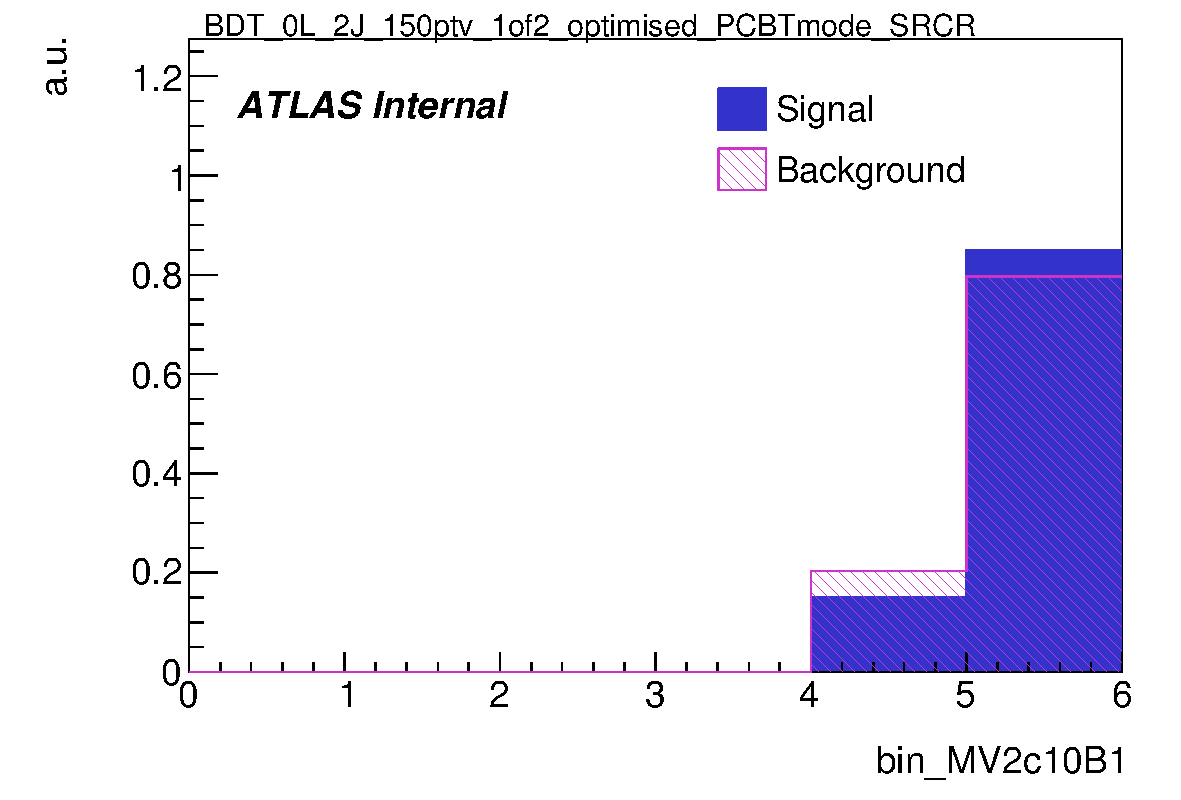
\includegraphics[width=0.33\linewidth]{0-lep-mva/Distr_SignalBackground_bin_MV2c10B1_BDT_0L_2J_150ptv_1of2_optimised_PCBTmode_SRCR-eps-converted-to}}
    \subfloat[]{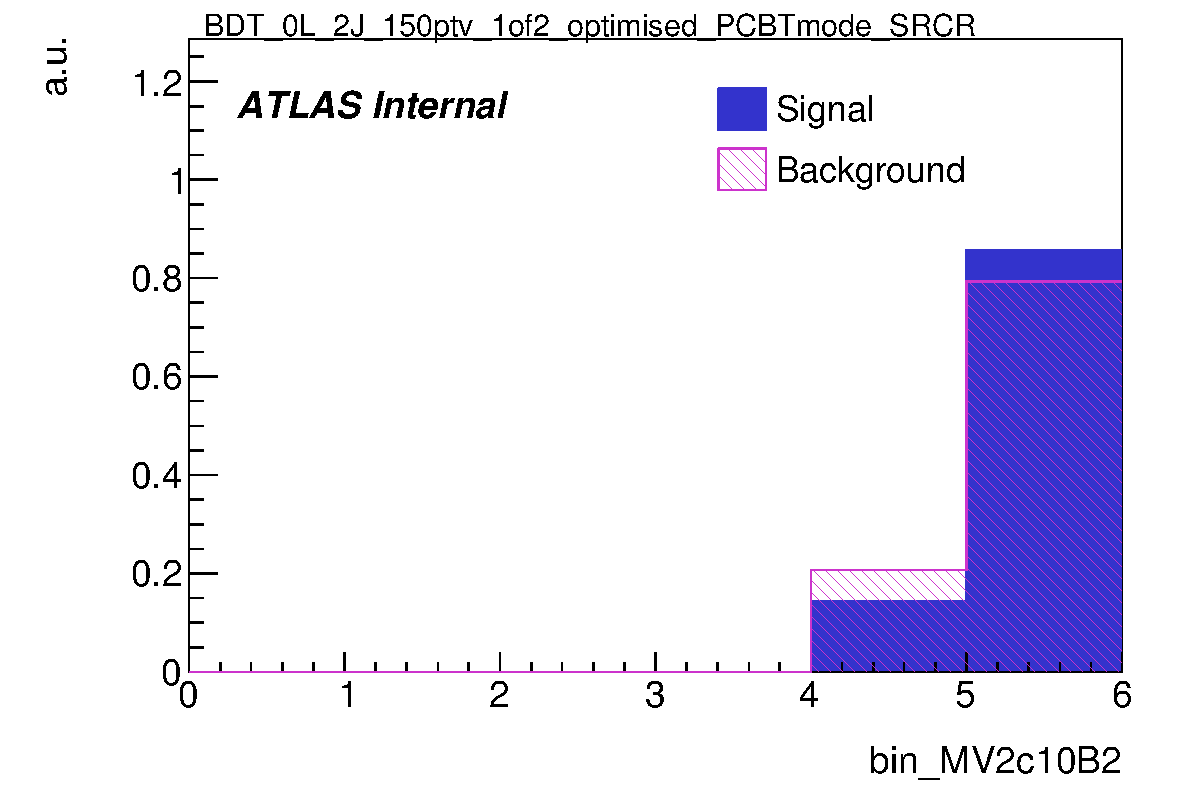
\includegraphics[width=0.33\linewidth]{0-lep-mva/Distr_SignalBackground_bin_MV2c10B2_BDT_0L_2J_150ptv_1of2_optimised_PCBTmode_SRCR-eps-converted-to}}
     \subfloat[]{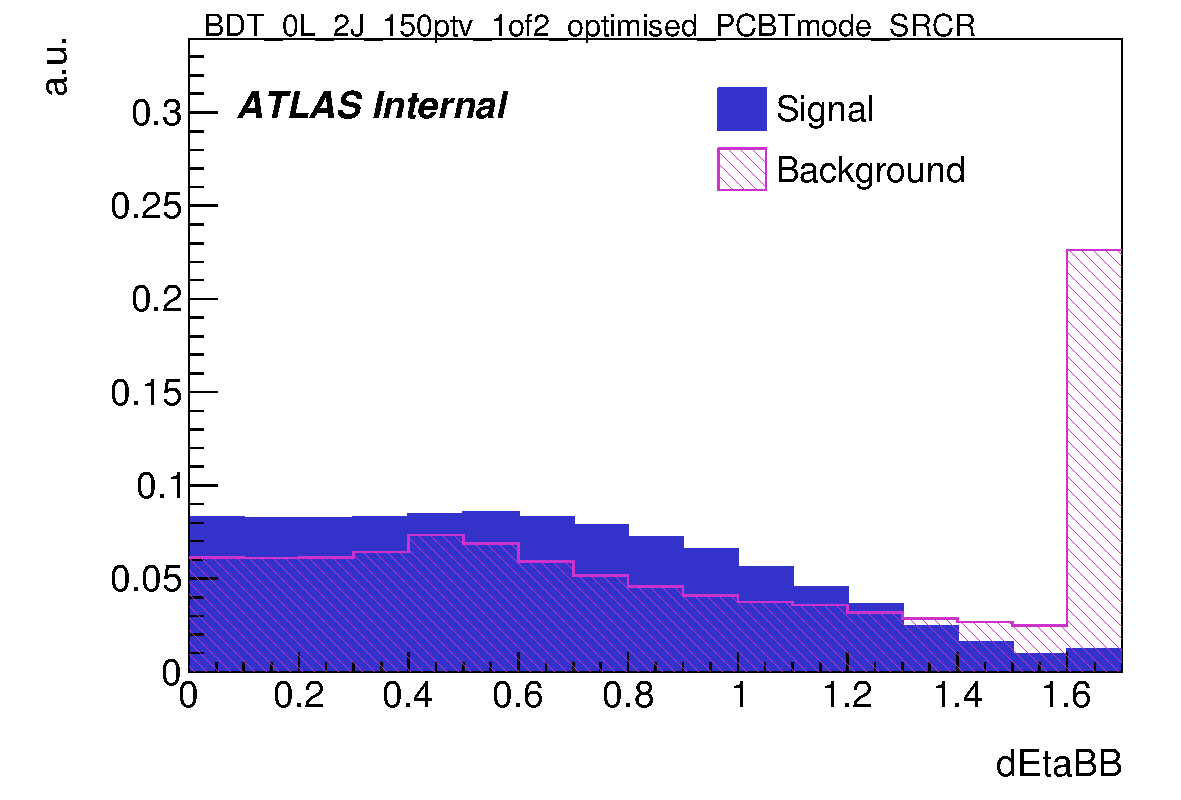
\includegraphics[width=0.33\linewidth]{0-lep-mva/Distr_SignalBackground_dEtaBB_BDT_0L_2J_150ptv_1of2_optimised_PCBTmode_SRCR-eps-converted-to}}\\
    \subfloat[]{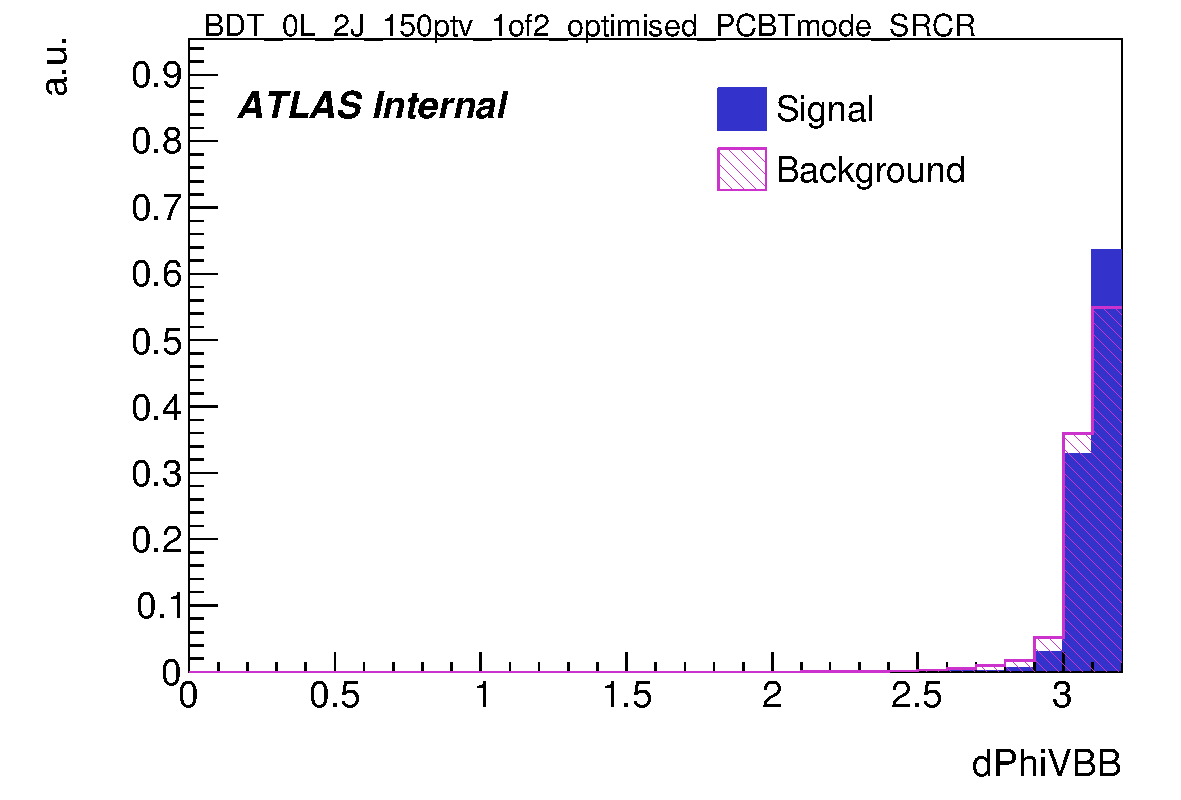
\includegraphics[width=0.33\linewidth]{0-lep-mva/Distr_SignalBackground_dPhiVBB_BDT_0L_2J_150ptv_1of2_optimised_PCBTmode_SRCR-eps-converted-to}}
    \subfloat[]{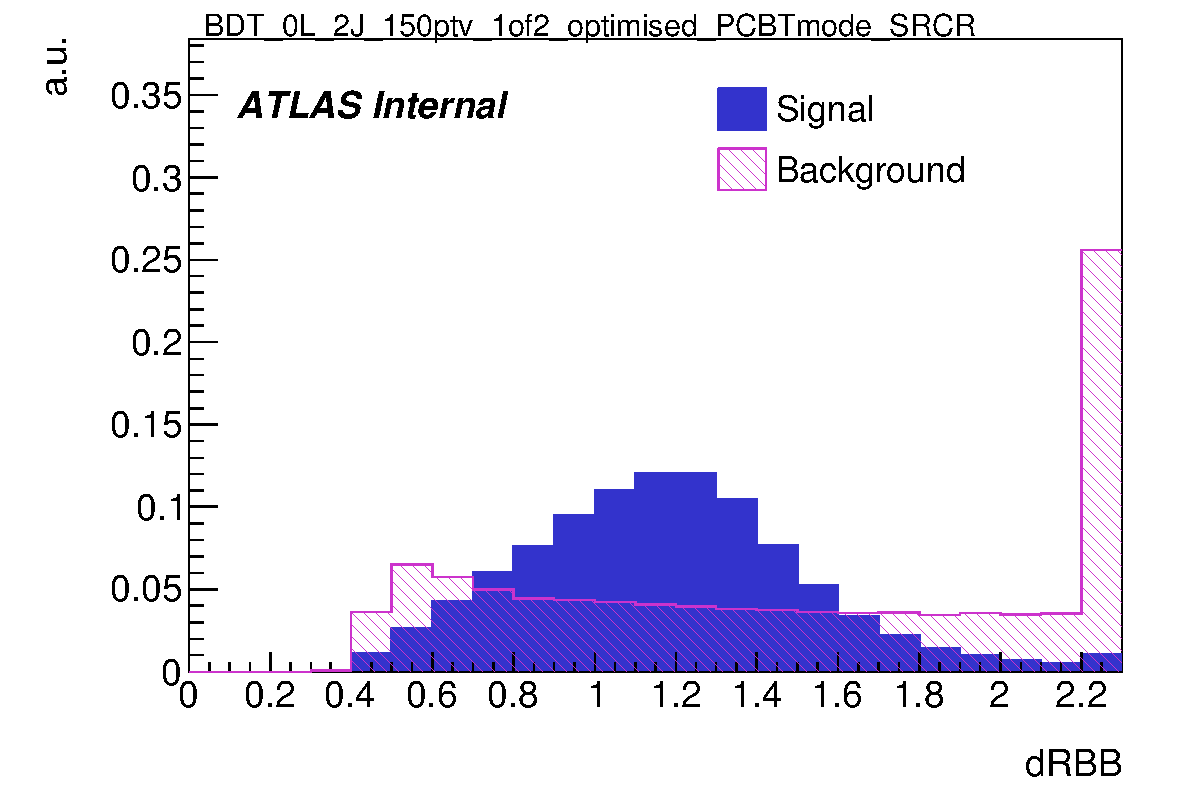
\includegraphics[width=0.33\linewidth]{0-lep-mva/Distr_SignalBackground_dRBB_BDT_0L_2J_150ptv_1of2_optimised_PCBTmode_SRCR-eps-converted-to}}
     \subfloat[]{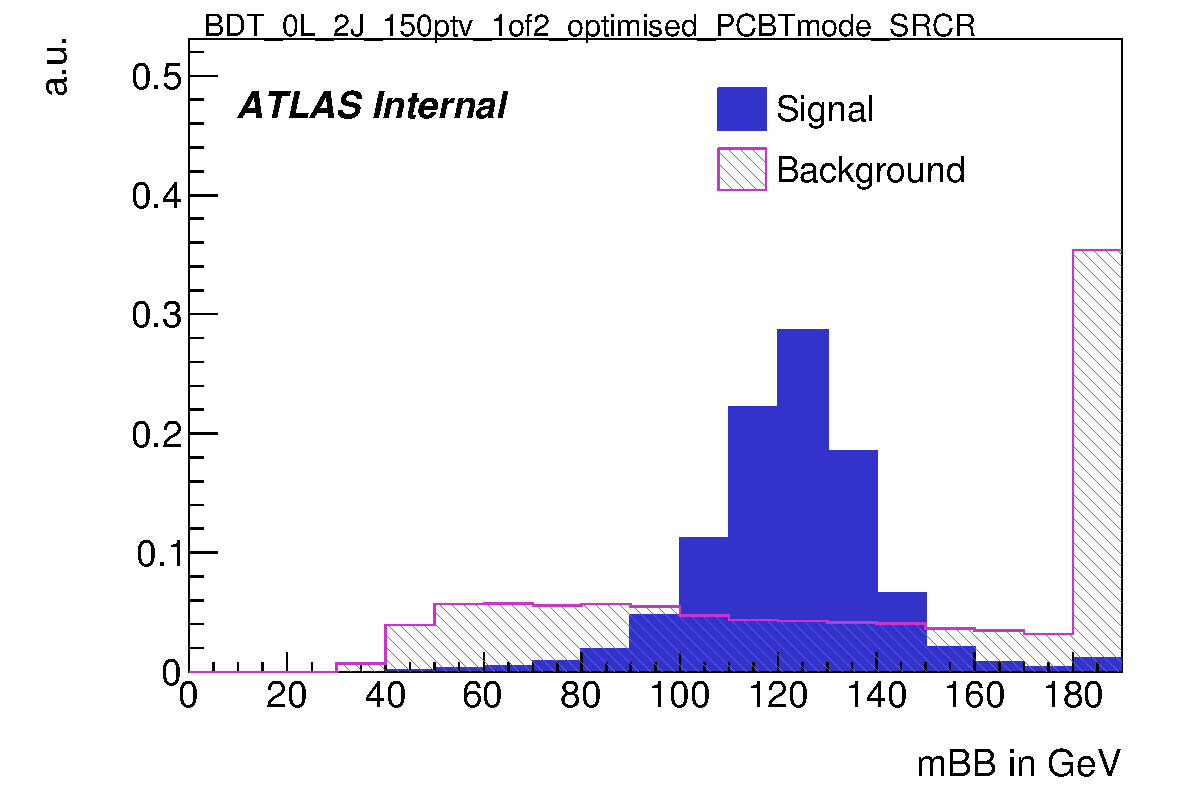
\includegraphics[width=0.33\linewidth]{0-lep-mva/Distr_SignalBackground_mBB_BDT_0L_2J_150ptv_1of2_optimised_PCBTmode_SRCR-eps-converted-to}}\\
    \subfloat[]{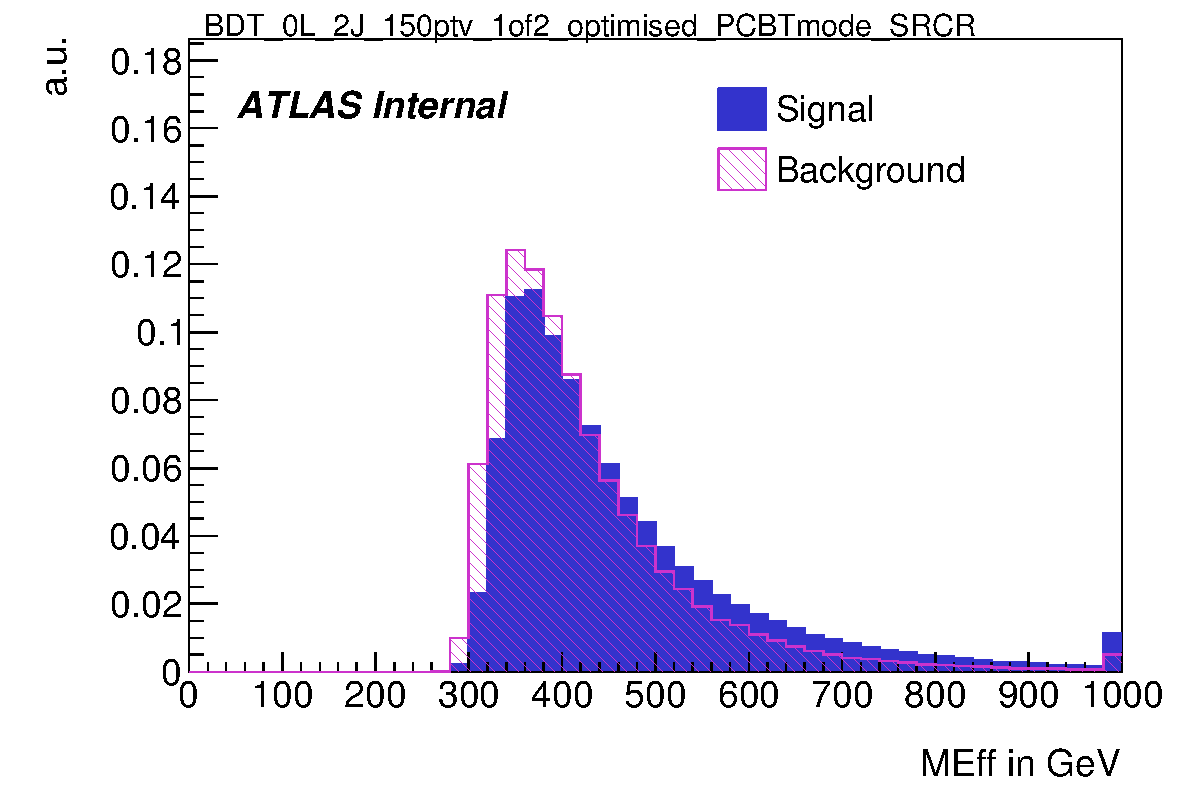
\includegraphics[width=0.33\linewidth]{0-lep-mva/Distr_SignalBackground_MEff_BDT_0L_2J_150ptv_1of2_optimised_PCBTmode_SRCR-eps-converted-to}}
     \subfloat[]{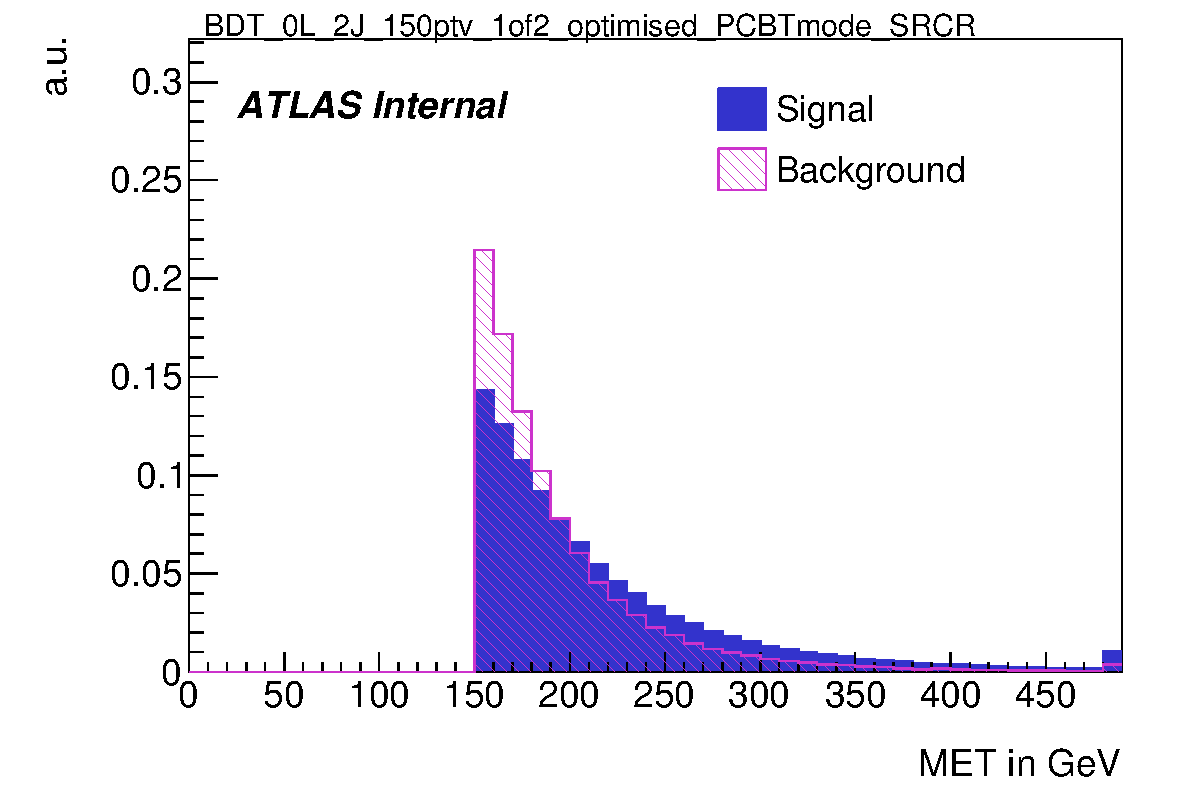
\includegraphics[width=0.33\linewidth]{0-lep-mva/Distr_SignalBackground_MET_BDT_0L_2J_150ptv_1of2_optimised_PCBTmode_SRCR-eps-converted-to}}          
    \subfloat[]{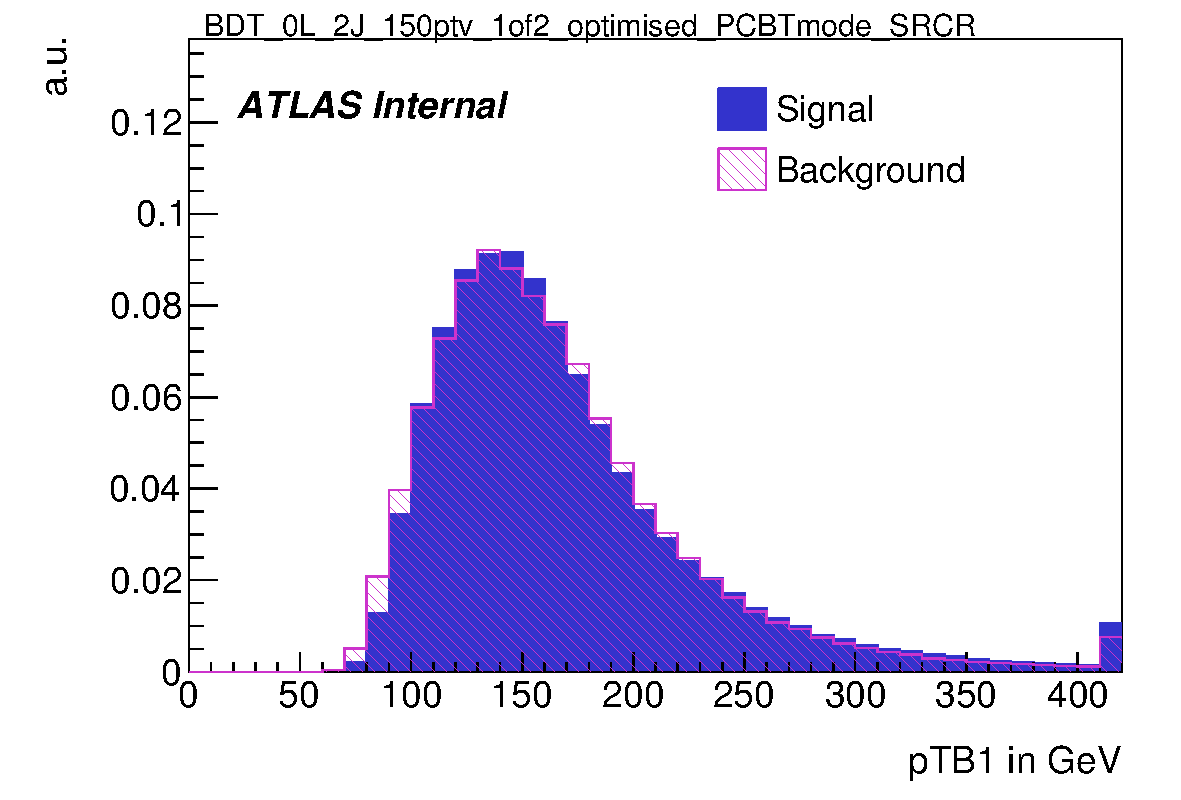
\includegraphics[width=0.33\linewidth]{0-lep-mva/Distr_SignalBackground_pTB1_BDT_0L_2J_150ptv_1of2_optimised_PCBTmode_SRCR-eps-converted-to}} \\
    \subfloat[]{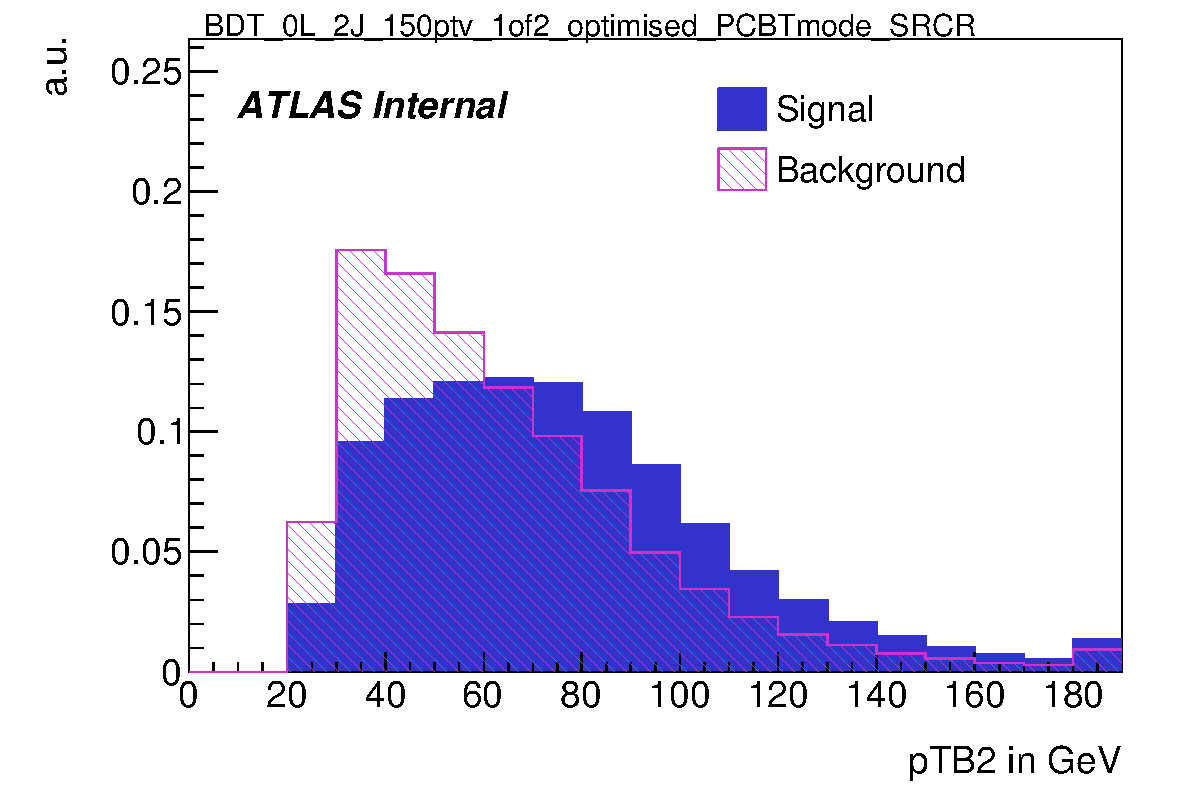
\includegraphics[width=0.33\linewidth]{0-lep-mva/Distr_SignalBackground_pTB2_BDT_0L_2J_150ptv_1of2_optimised_PCBTmode_SRCR-eps-converted-to}}   
    \subfloat[]{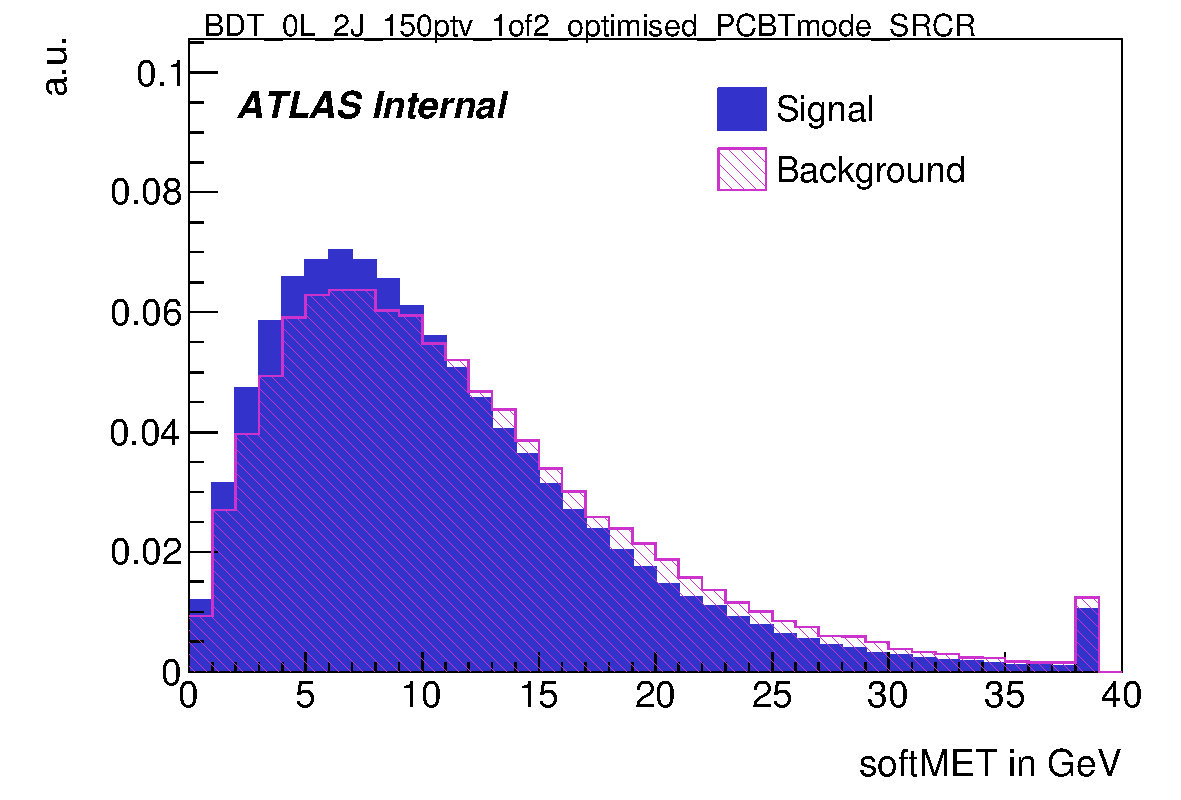
\includegraphics[width=0.33\linewidth]{0-lep-mva/Distr_SignalBackground_softMET_BDT_0L_2J_150ptv_1of2_optimised_PCBTmode_SRCR-eps-converted-to}}\\    
    \end{tabular}
    \caption{Input variables passed to the BDT for sum of all signal (blue) and sum of all background (red) samples in the 0 lepton channel for the 2 jet region with $E_T^{miss}>$150 {GeV} are shown. The signal and background templates are normalised to the same yield. The variable range for the training is restricted to contain 99\% of all signal events and the events in the overflow are included in the last bin.}
    \label{fig:bdtinputs0L2J150}
\end{figure}

 \begin{figure}[htbp]
  \centering
  \begin{tabular}{cccc}
    \subfloat[]{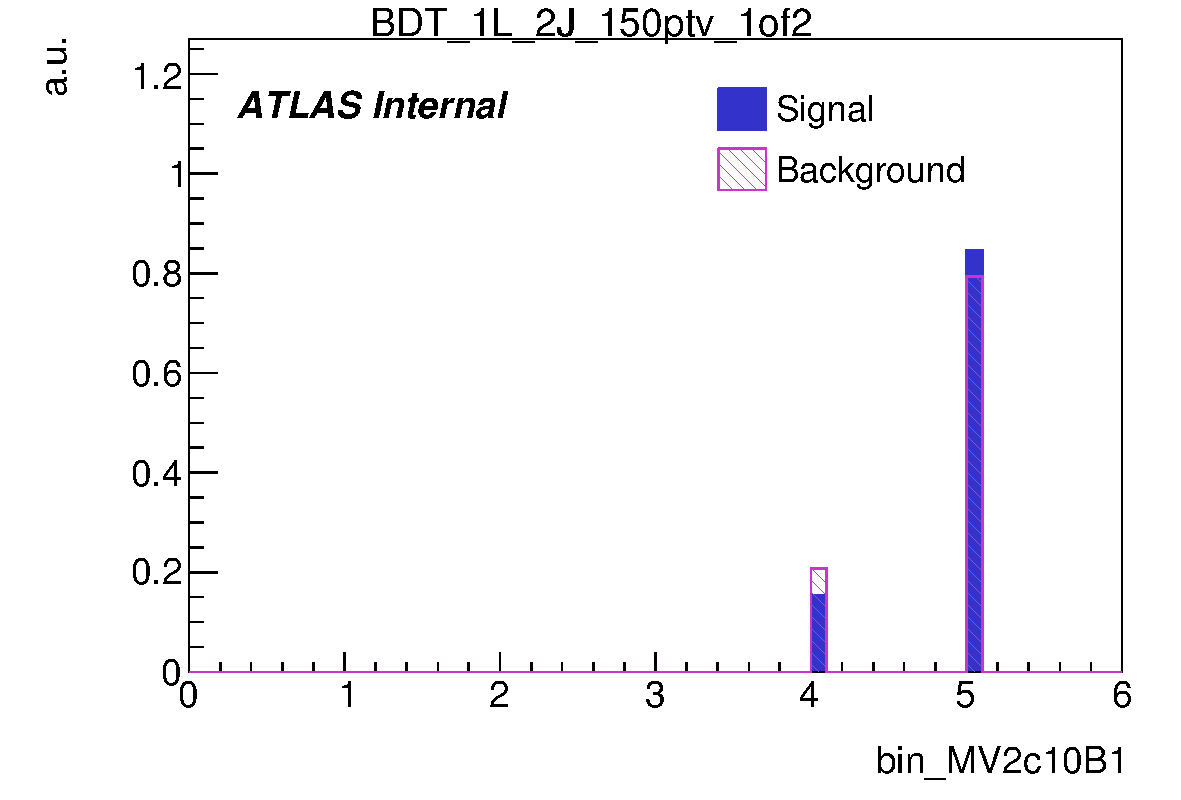
\includegraphics[width=0.3\linewidth]{1-lep-mva/Distr_SignalBackground_bin_MV2c10B1_BDT_1L_2J_150ptv_1of2-eps-converted-to}}
    \subfloat[]{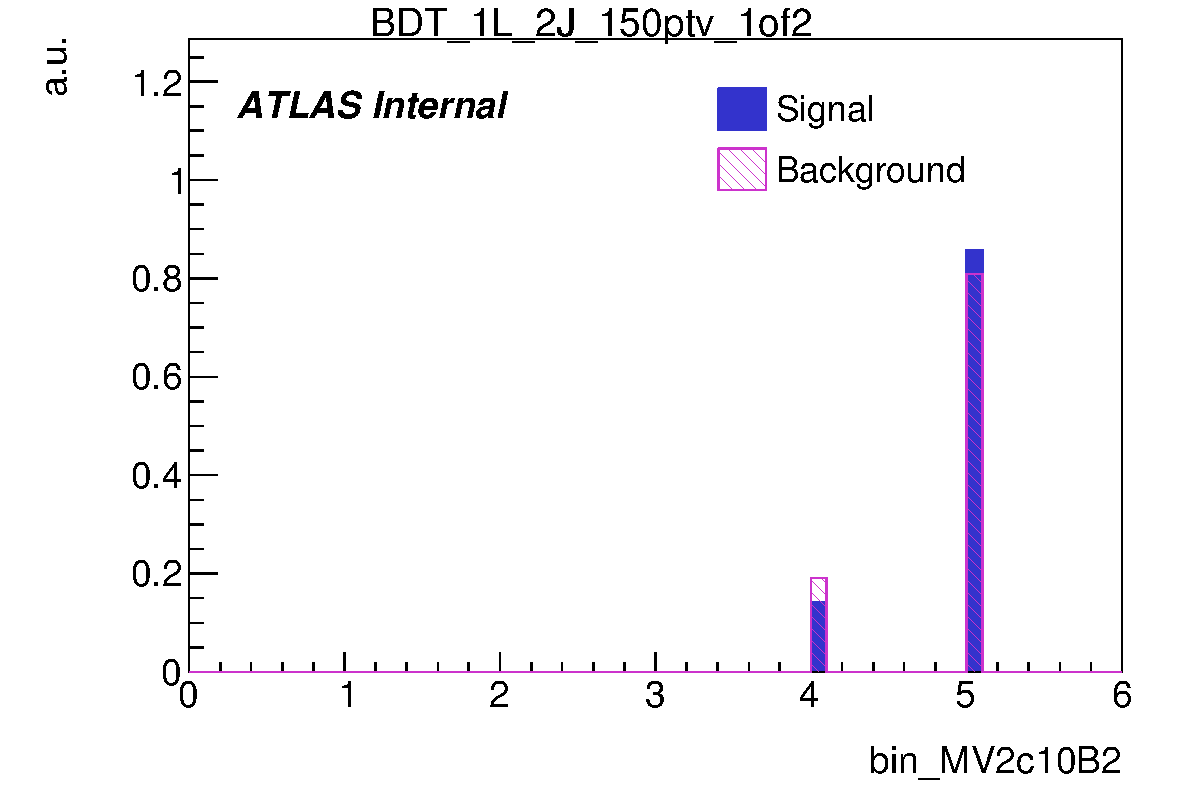
\includegraphics[width=0.3\linewidth]{1-lep-mva/Distr_SignalBackground_bin_MV2c10B2_BDT_1L_2J_150ptv_1of2-eps-converted-to}}
     \subfloat[]{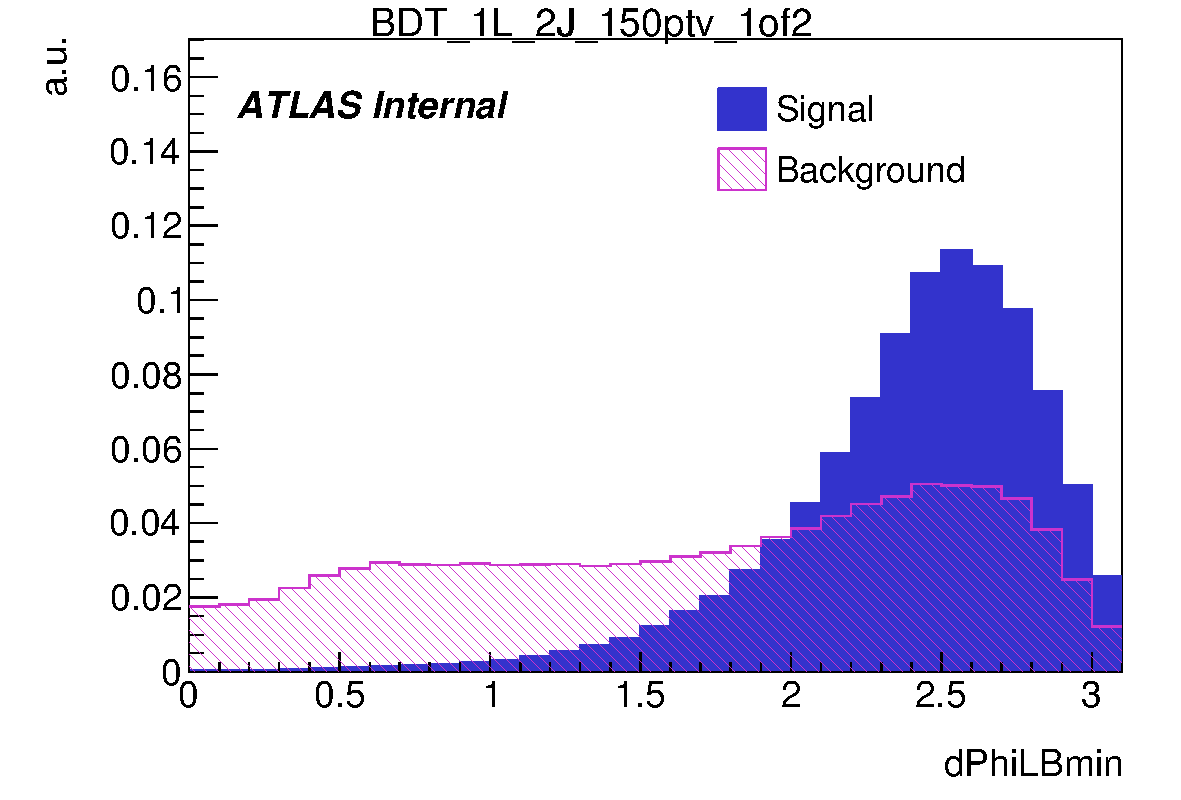
\includegraphics[width=0.3\linewidth]{1-lep-mva/Distr_SignalBackground_dPhiLBmin_BDT_1L_2J_150ptv_1of2-eps-converted-to}}\\
    \subfloat[]{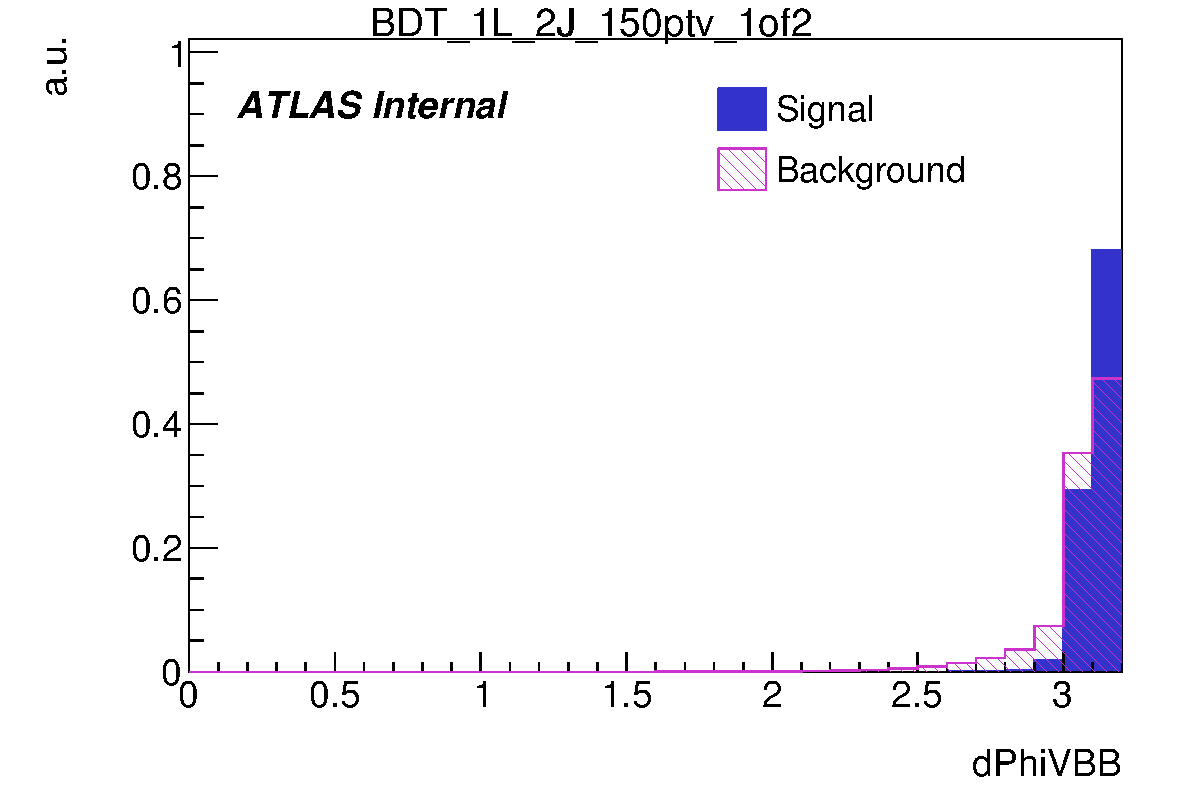
\includegraphics[width=0.3\linewidth]{1-lep-mva/Distr_SignalBackground_dPhiVBB_BDT_1L_2J_150ptv_1of2-eps-converted-to}}
    \subfloat[]{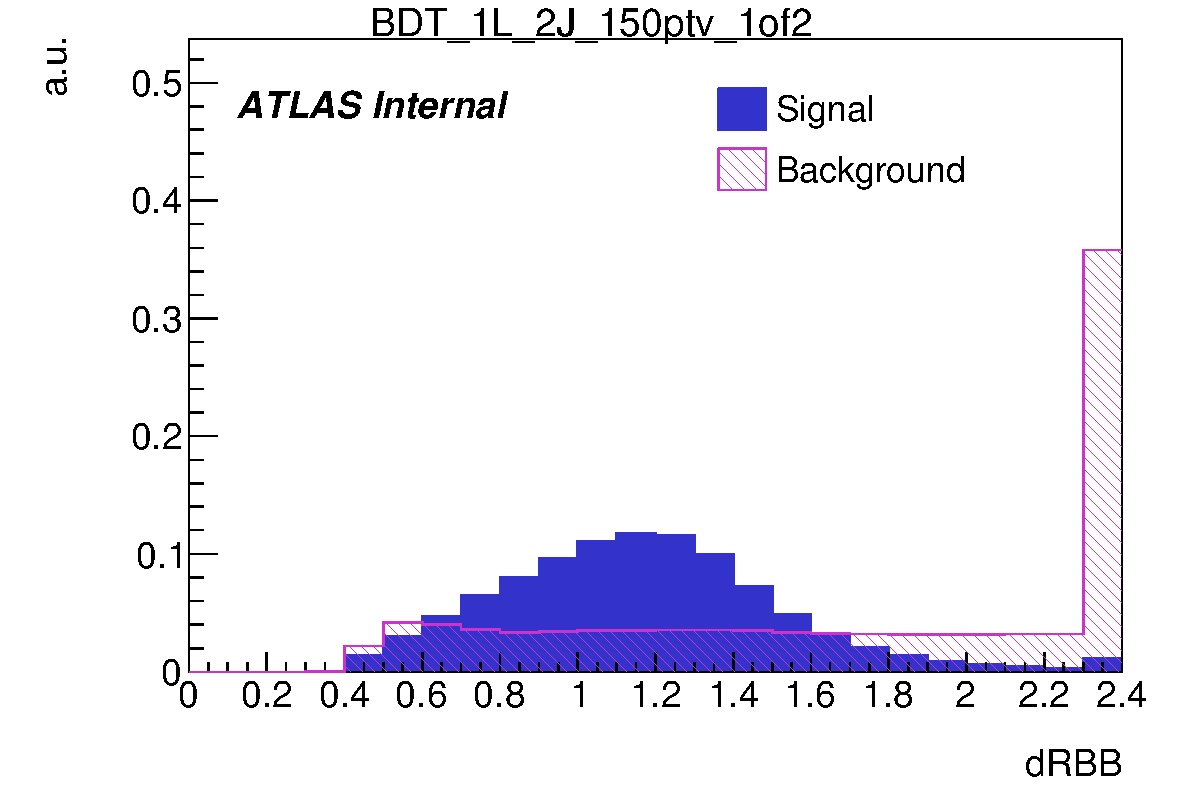
\includegraphics[width=0.3\linewidth]{1-lep-mva/Distr_SignalBackground_dRBB_BDT_1L_2J_150ptv_1of2-eps-converted-to}}
     \subfloat[]{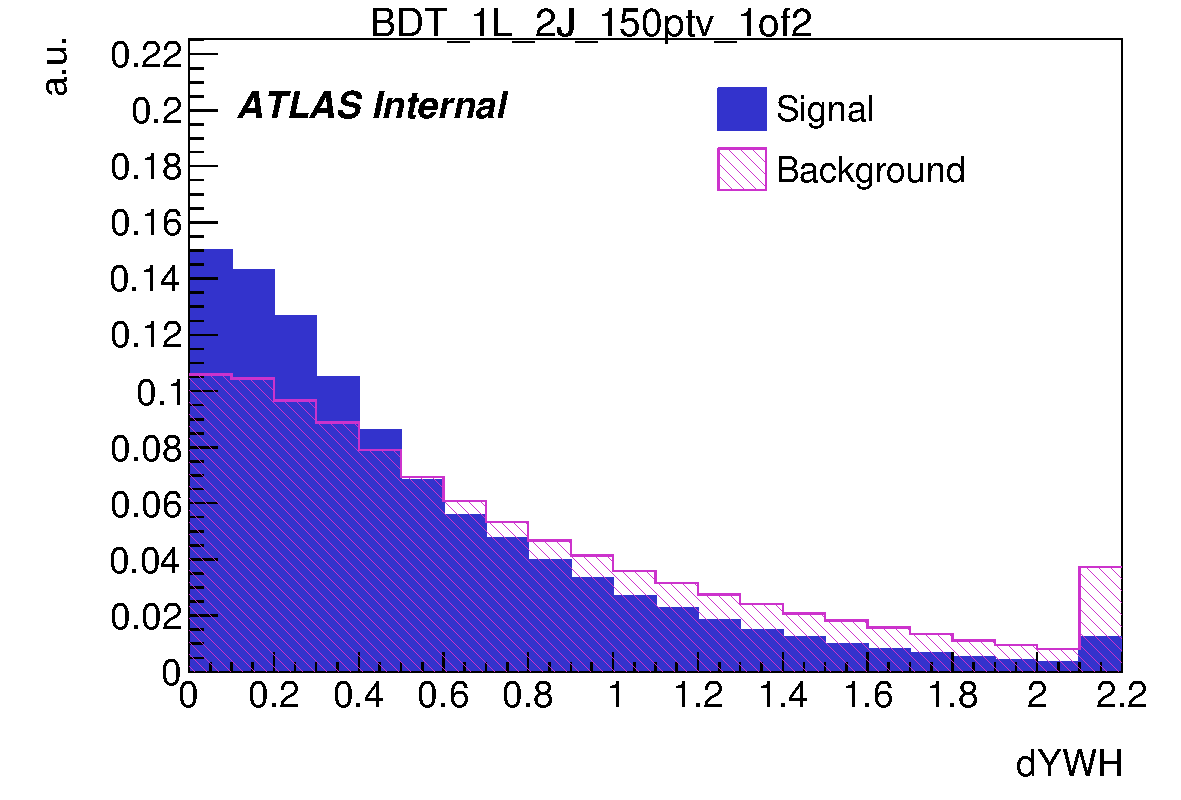
\includegraphics[width=0.3\linewidth]{1-lep-mva/Distr_SignalBackground_dYWH_BDT_1L_2J_150ptv_1of2-eps-converted-to}}\\
    \subfloat[]{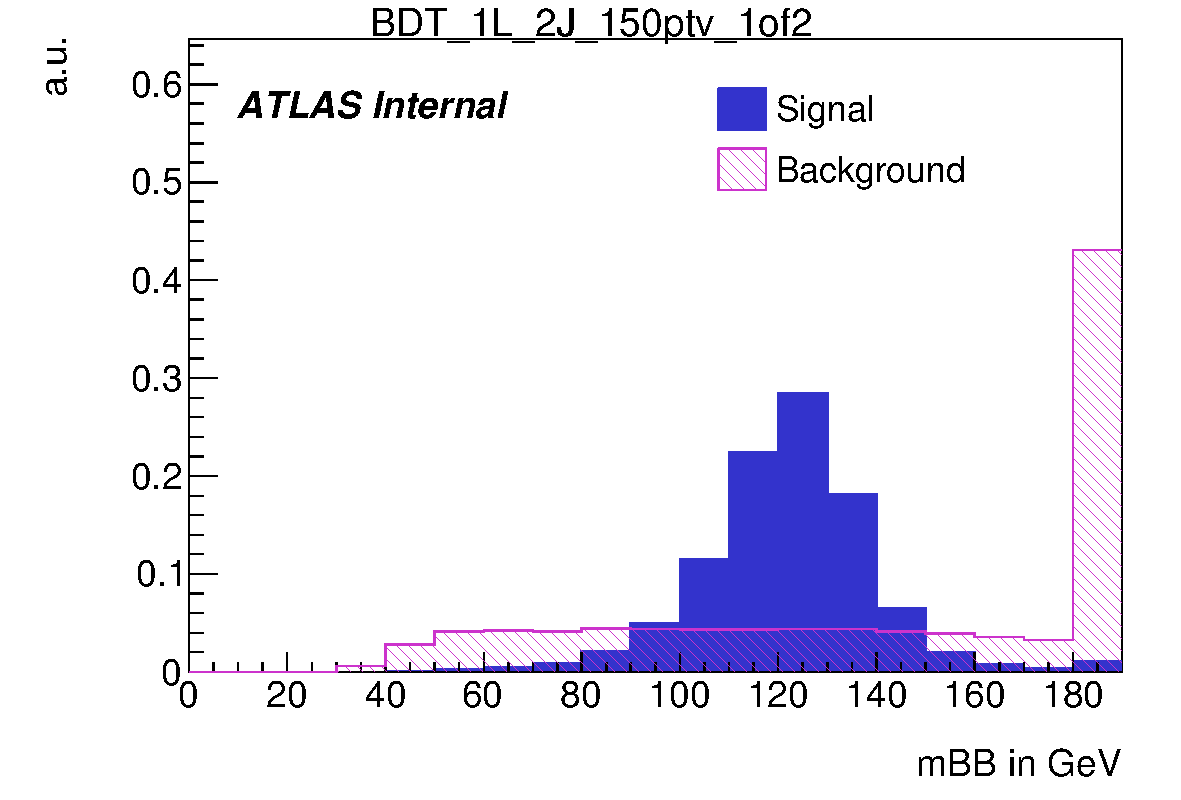
\includegraphics[width=0.3\linewidth]{1-lep-mva/Distr_SignalBackground_mBB_BDT_1L_2J_150ptv_1of2-eps-converted-to}}
     \subfloat[]{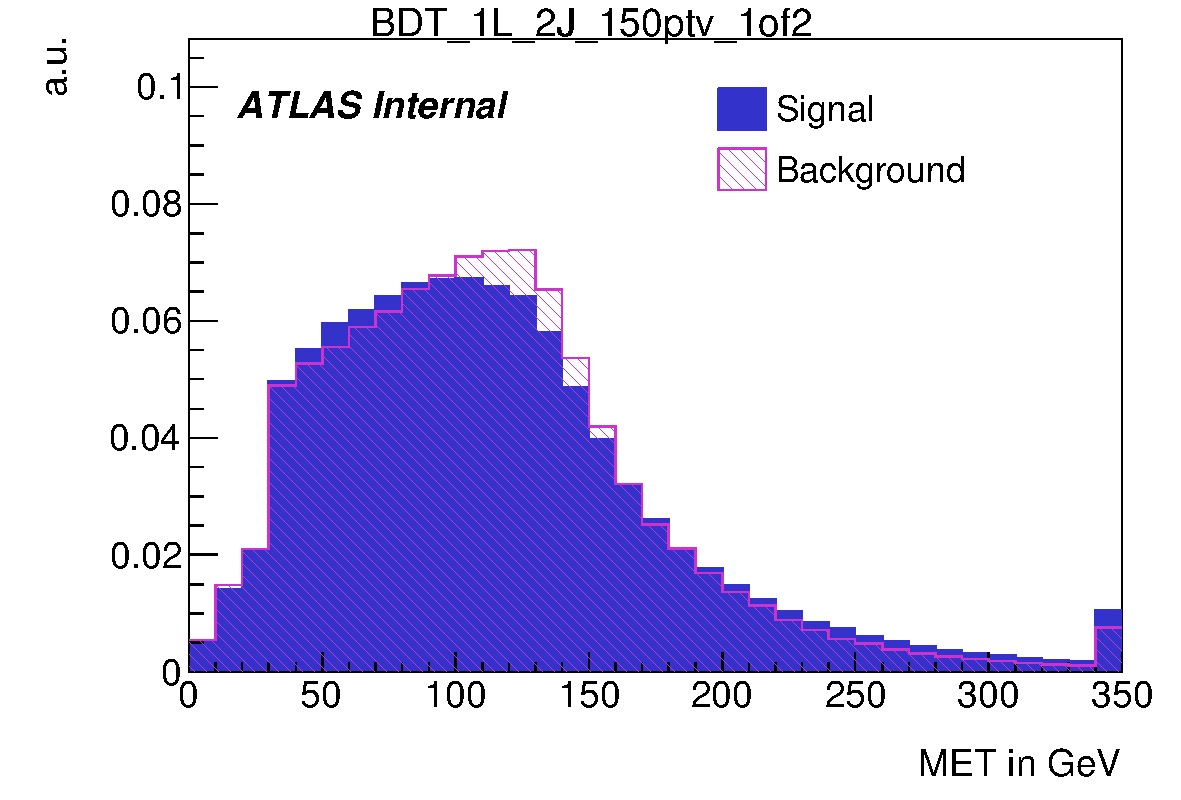
\includegraphics[width=0.3\linewidth]{1-lep-mva/Distr_SignalBackground_MET_BDT_1L_2J_150ptv_1of2-eps-converted-to}}          
    \subfloat[]{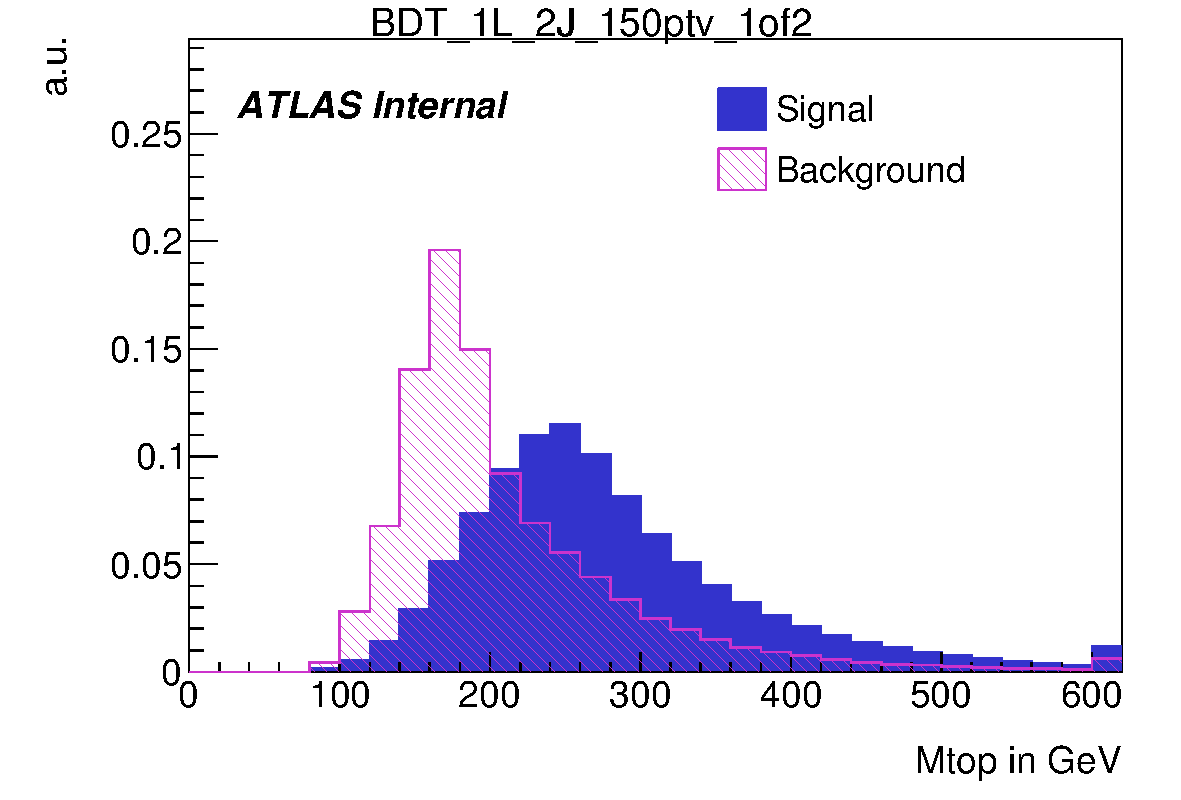
\includegraphics[width=0.3\linewidth]{1-lep-mva/Distr_SignalBackground_Mtop_BDT_1L_2J_150ptv_1of2-eps-converted-to}} \\
    \subfloat[]{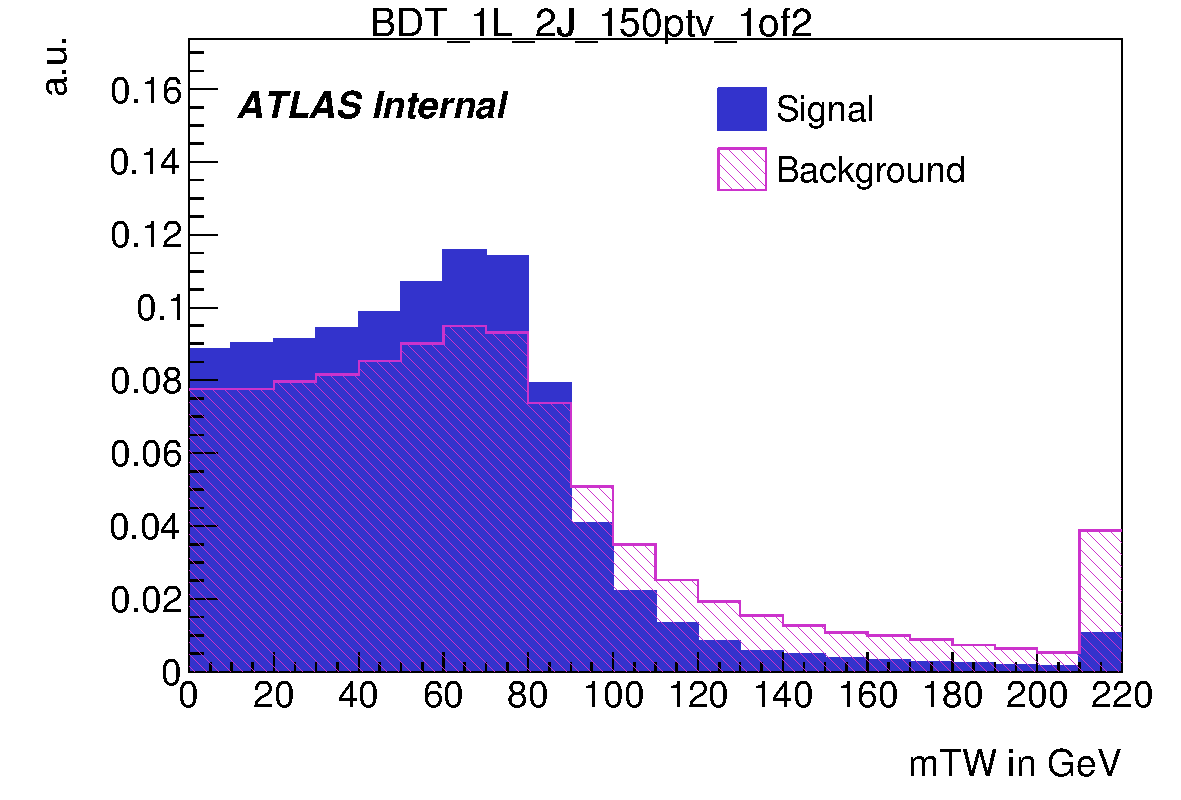
\includegraphics[width=0.3\linewidth]{1-lep-mva/Distr_SignalBackground_mTW_BDT_1L_2J_150ptv_1of2-eps-converted-to}}   
    \subfloat[]{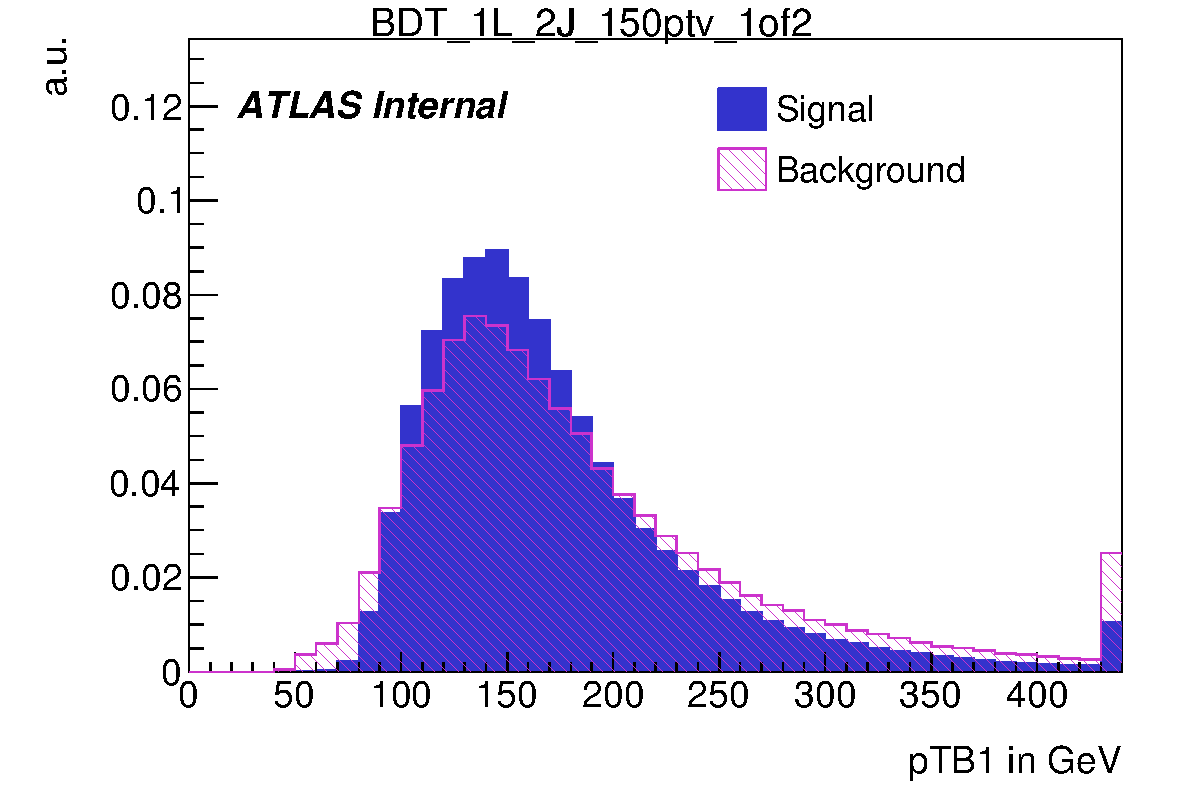
\includegraphics[width=0.3\linewidth]{1-lep-mva/Distr_SignalBackground_pTB1_BDT_1L_2J_150ptv_1of2-eps-converted-to}}
    \subfloat[]{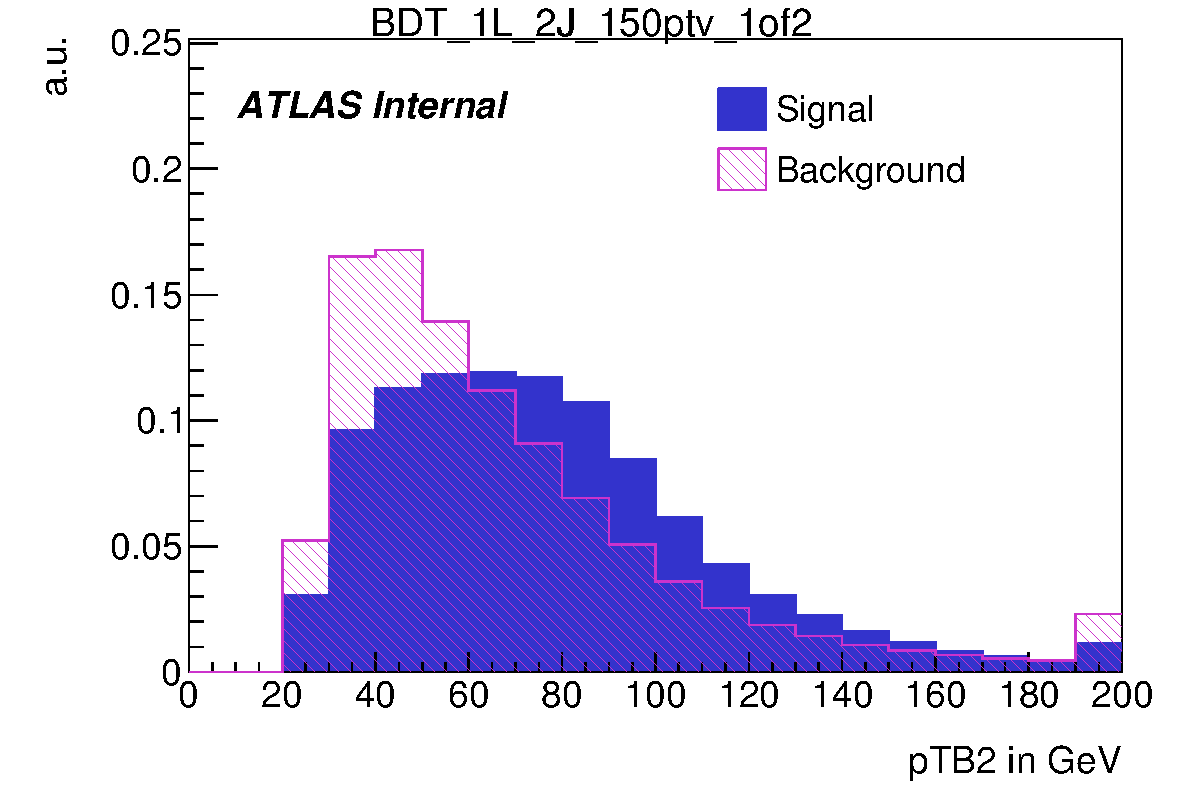
\includegraphics[width=0.3\linewidth]{1-lep-mva/Distr_SignalBackground_pTB2_BDT_1L_2J_150ptv_1of2-eps-converted-to}}\\   
    \subfloat[]{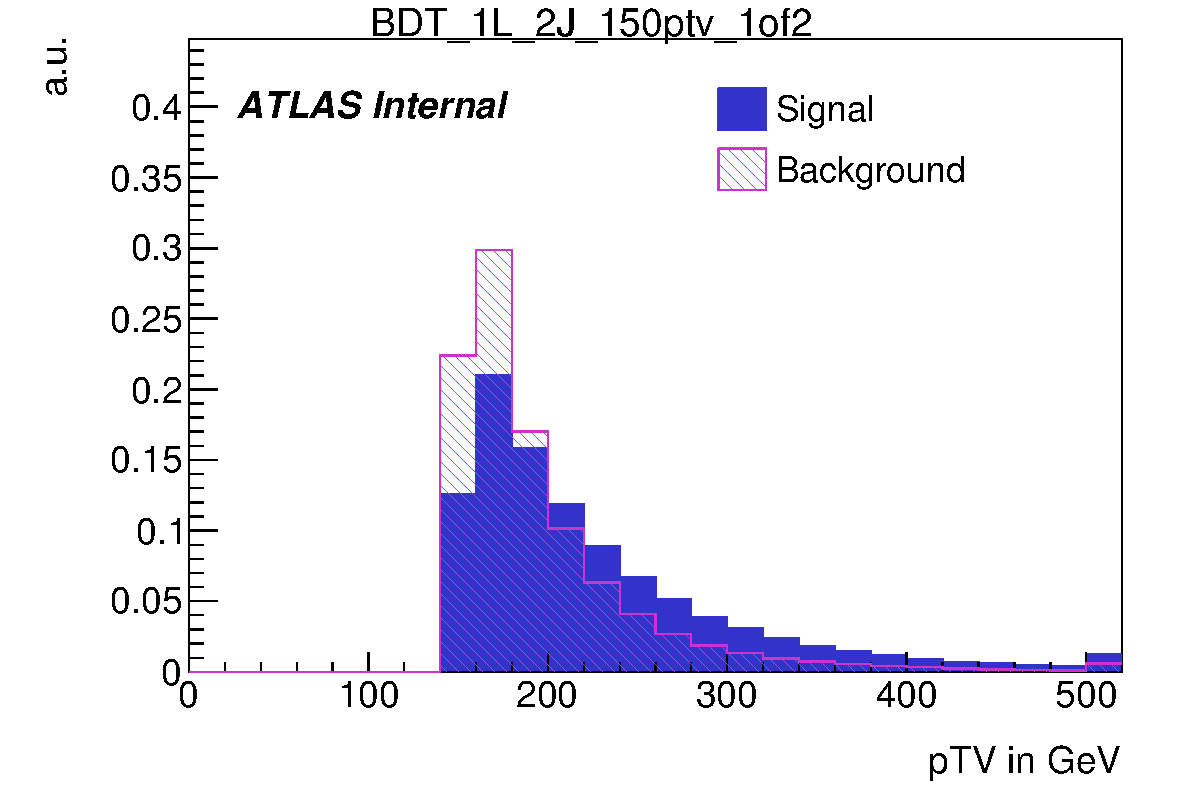
\includegraphics[width=0.3\linewidth]{1-lep-mva/Distr_SignalBackground_pTV_BDT_1L_2J_150ptv_1of2-eps-converted-to}} 
    \end{tabular}
    \caption{Input variables passed to the BDT for sum of all signal (blue) and sum of all background (red) samples in the 1 lepton channel for the 2 jet region with $p_{\text{T}}^{W}>$150 {GeV} are shown. The signal and background templates are normalised to the same yield. The variable range for the training is restricted to contain 99\% of all signal events and the events in the overflow are included in the last bin.}
    \label{fig:bdtinputs1L2J150New}
\end{figure}

 \begin{figure}[htbp]
  \centering
  \begin{tabular}{cccc}
    \subfloat[]{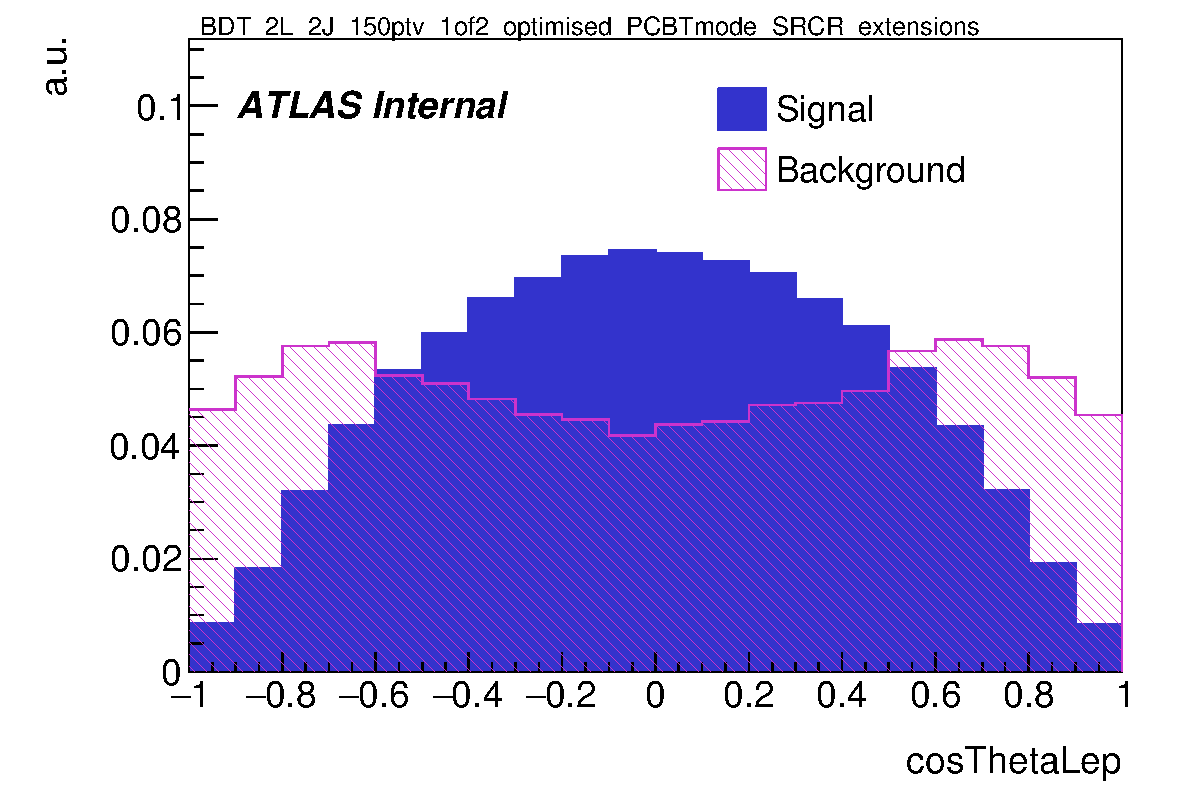
\includegraphics[width=0.33\linewidth]{2-lep-mva/Distr_SignalBackground_cosThetaLep_BDT_2L_2J_150ptv_1of2_optimised_PCBTmode_SRCR_extensions-eps-converted-to}}
    \subfloat[]{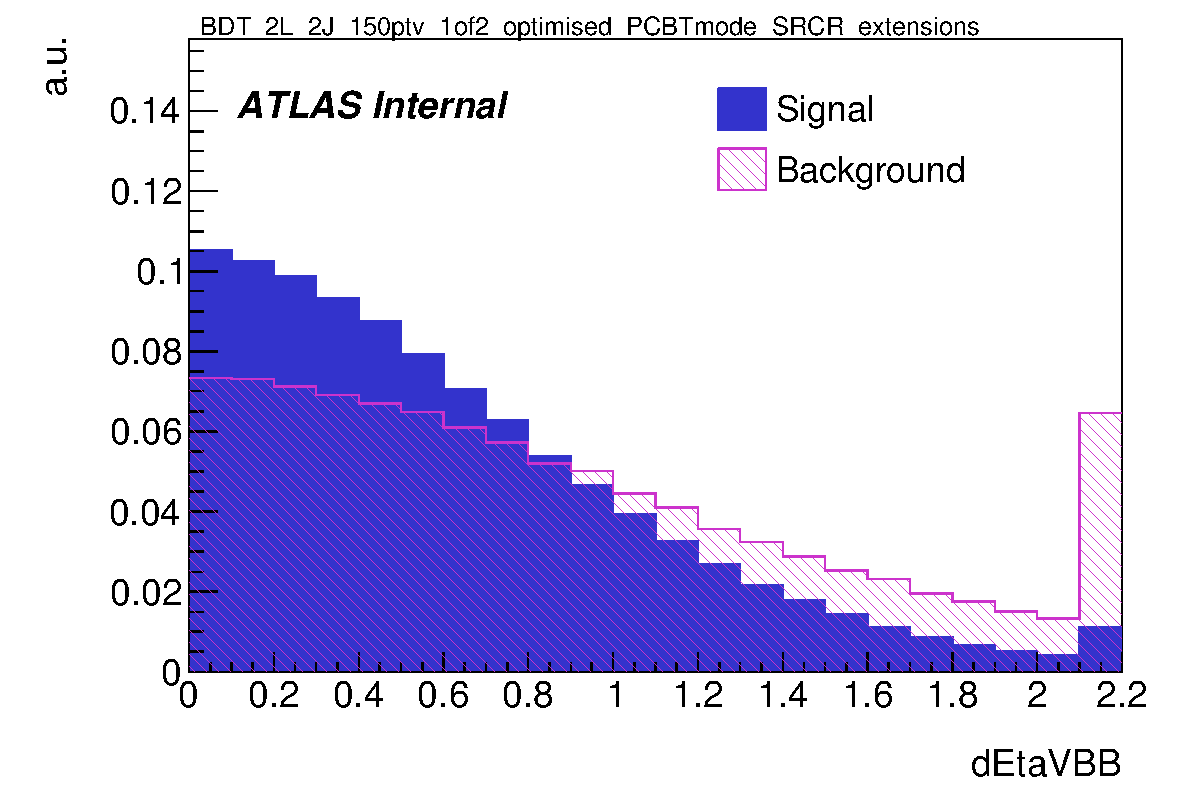
\includegraphics[width=0.33\linewidth]{2-lep-mva/Distr_SignalBackground_dEtaVBB_BDT_2L_2J_150ptv_1of2_optimised_PCBTmode_SRCR_extensions-eps-converted-to}}
     \subfloat[]{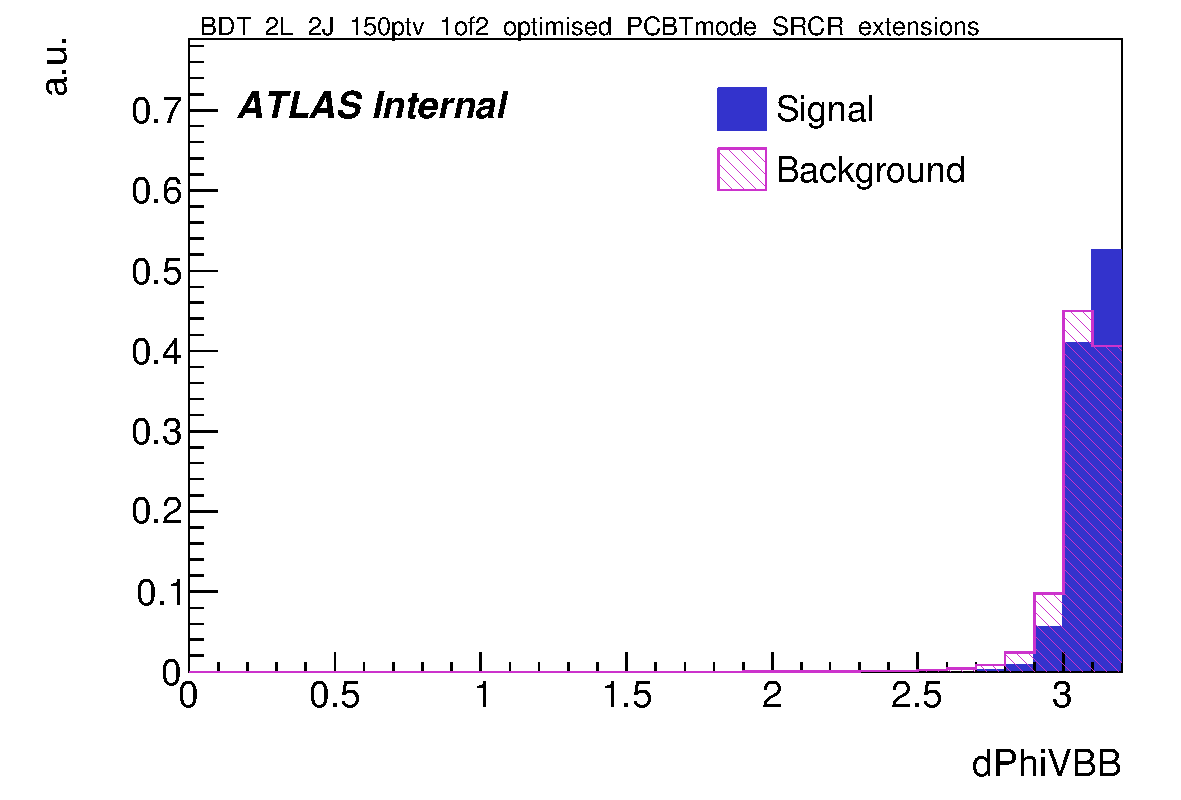
\includegraphics[width=0.33\linewidth]{2-lep-mva/Distr_SignalBackground_dPhiVBB_BDT_2L_2J_150ptv_1of2_optimised_PCBTmode_SRCR_extensions-eps-converted-to}}\\
    \subfloat[]{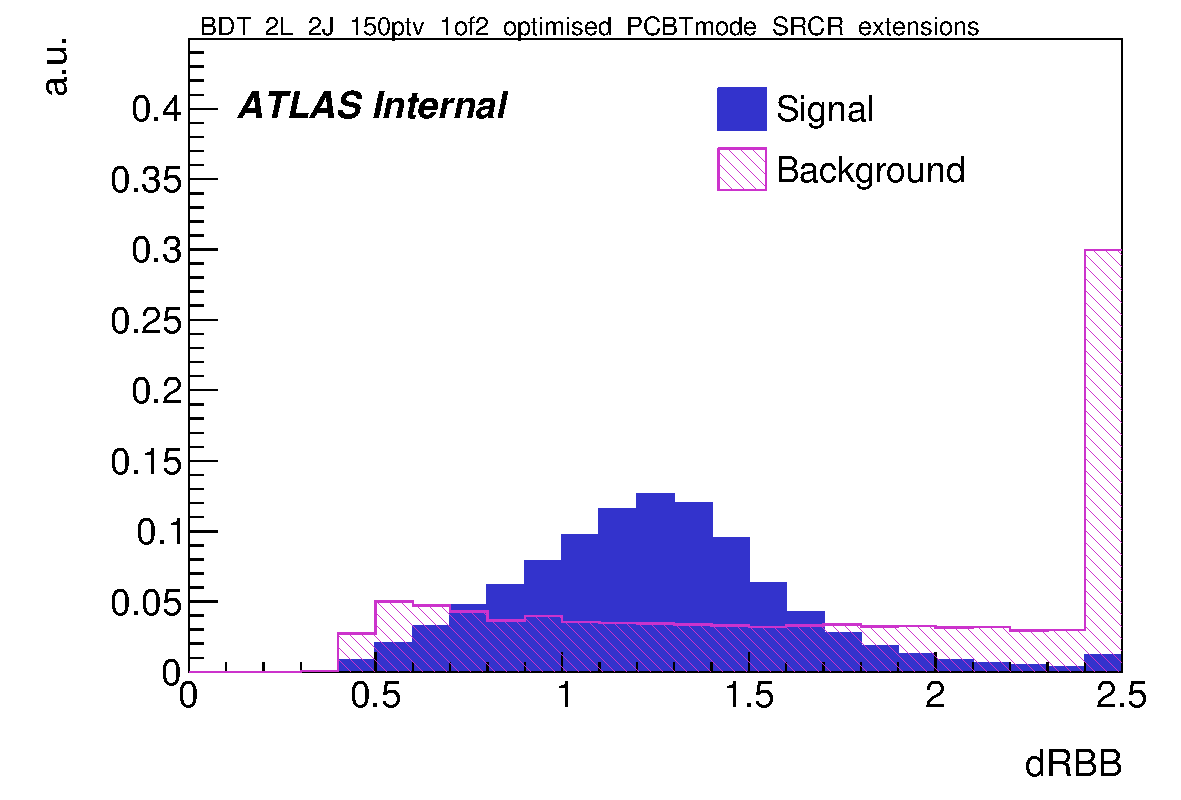
\includegraphics[width=0.33\linewidth]{2-lep-mva/Distr_SignalBackground_dRBB_BDT_2L_2J_150ptv_1of2_optimised_PCBTmode_SRCR_extensions-eps-converted-to}}
    \subfloat[]{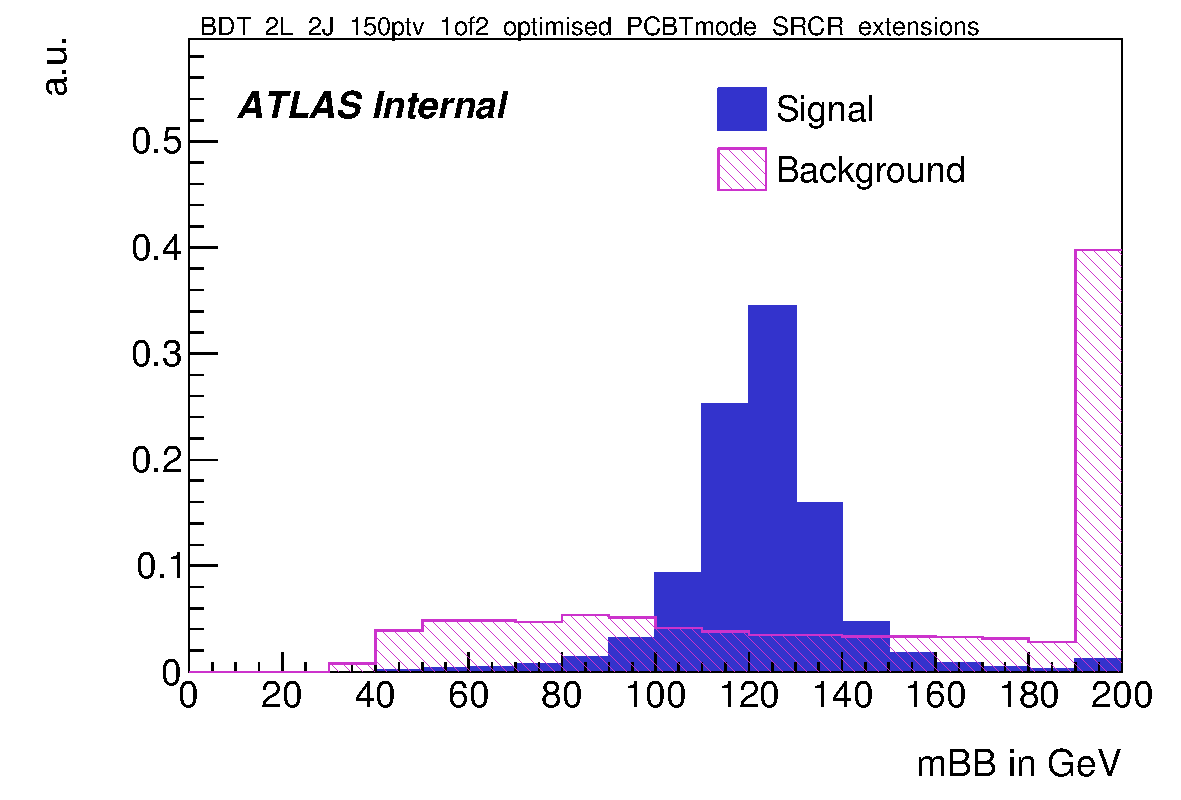
\includegraphics[width=0.33\linewidth]{2-lep-mva/Distr_SignalBackground_mBB_BDT_2L_2J_150ptv_1of2_optimised_PCBTmode_SRCR_extensions-eps-converted-to}}
     \subfloat[]{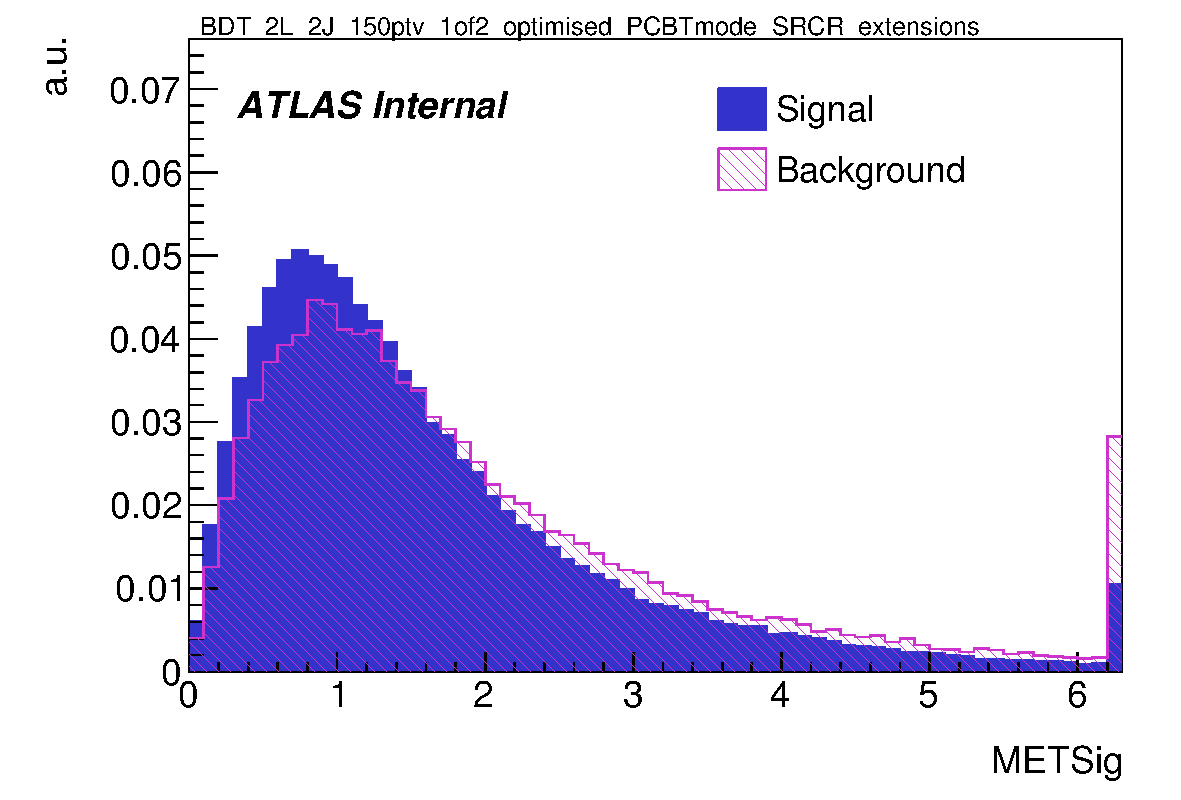
\includegraphics[width=0.33\linewidth]{2-lep-mva/Distr_SignalBackground_METSig_BDT_2L_2J_150ptv_1of2_optimised_PCBTmode_SRCR_extensions-eps-converted-to}}\\
    \subfloat[]{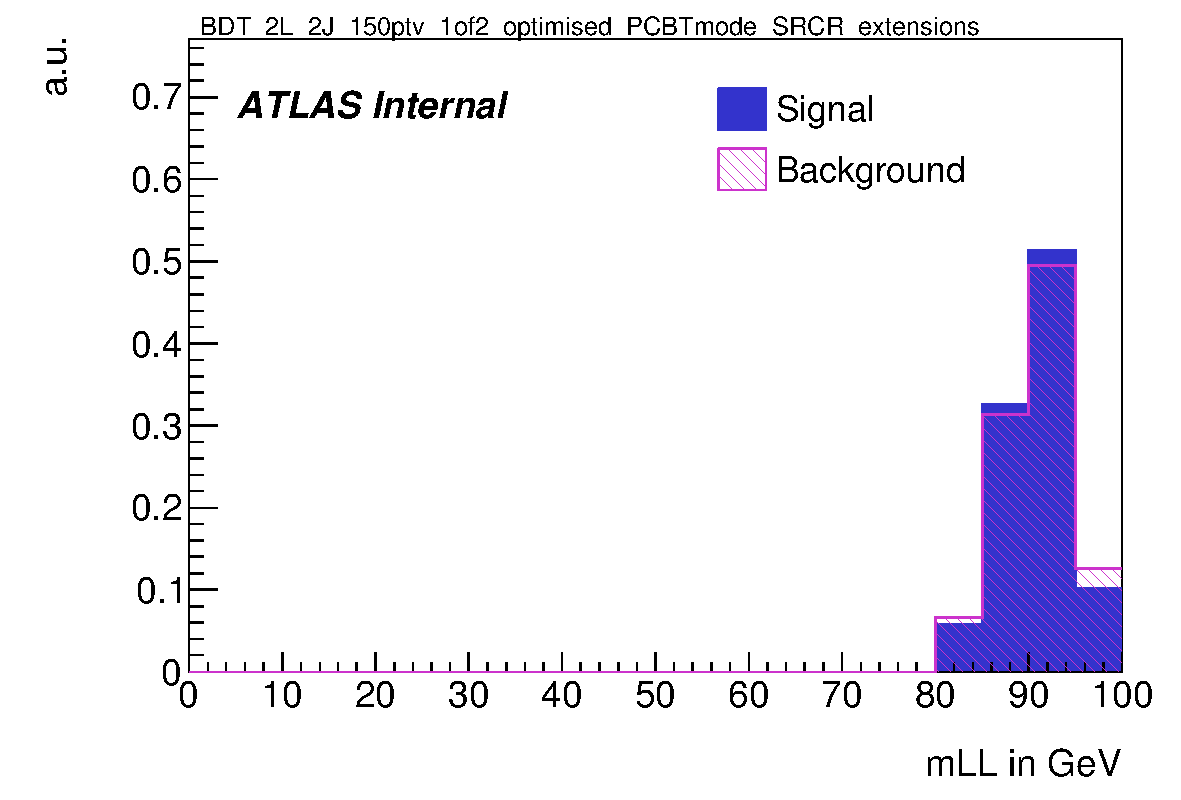
\includegraphics[width=0.33\linewidth]{2-lep-mva/Distr_SignalBackground_mLL_BDT_2L_2J_150ptv_1of2_optimised_PCBTmode_SRCR_extensions-eps-converted-to}}
     \subfloat[]{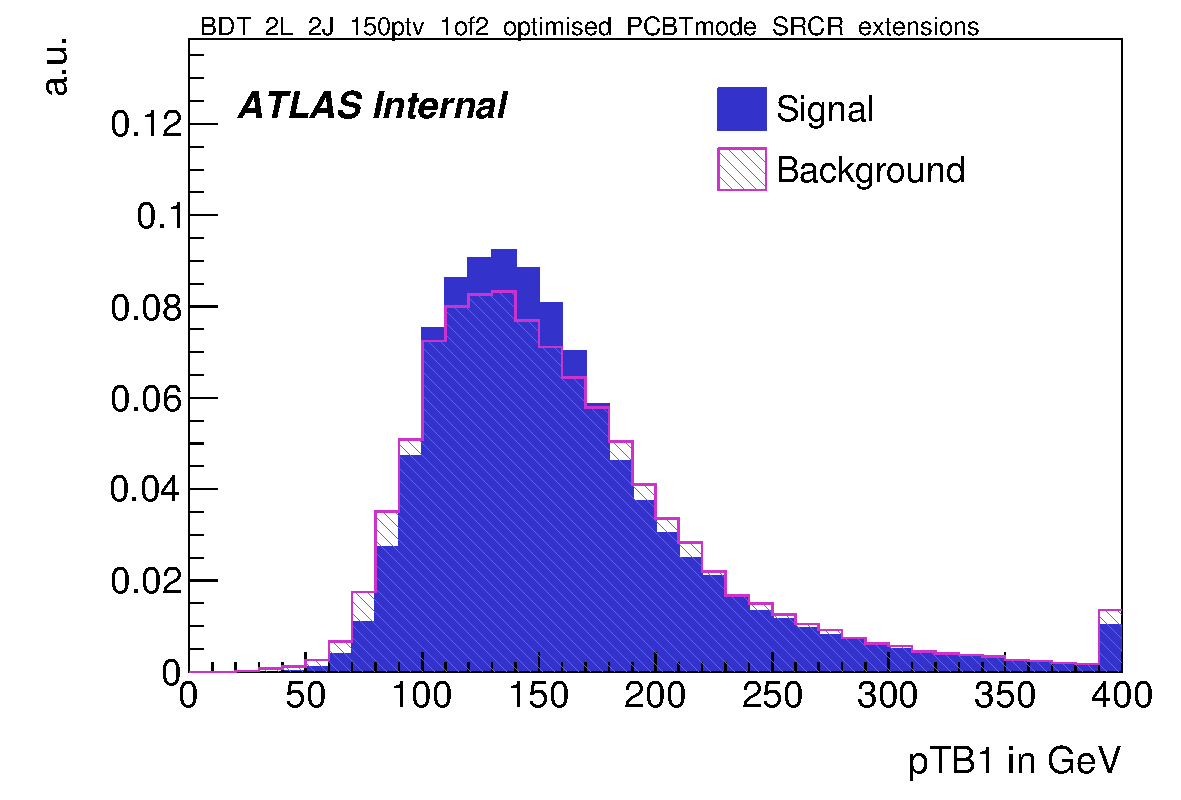
\includegraphics[width=0.33\linewidth]{2-lep-mva/Distr_SignalBackground_pTB1_BDT_2L_2J_150ptv_1of2_optimised_PCBTmode_SRCR_extensions-eps-converted-to}}          
    \subfloat[]{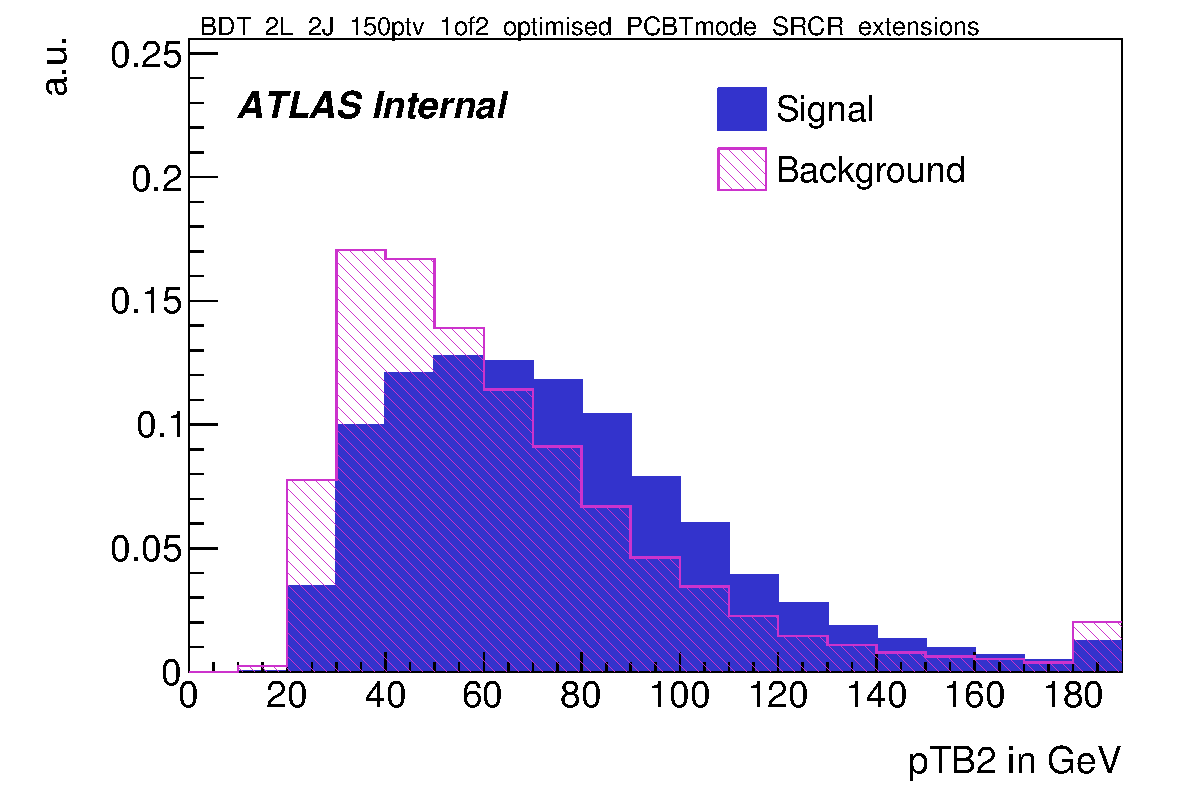
\includegraphics[width=0.33\linewidth]{2-lep-mva/Distr_SignalBackground_pTB2_BDT_2L_2J_150ptv_1of2_optimised_PCBTmode_SRCR_extensions-eps-converted-to}} \\
    \subfloat[]{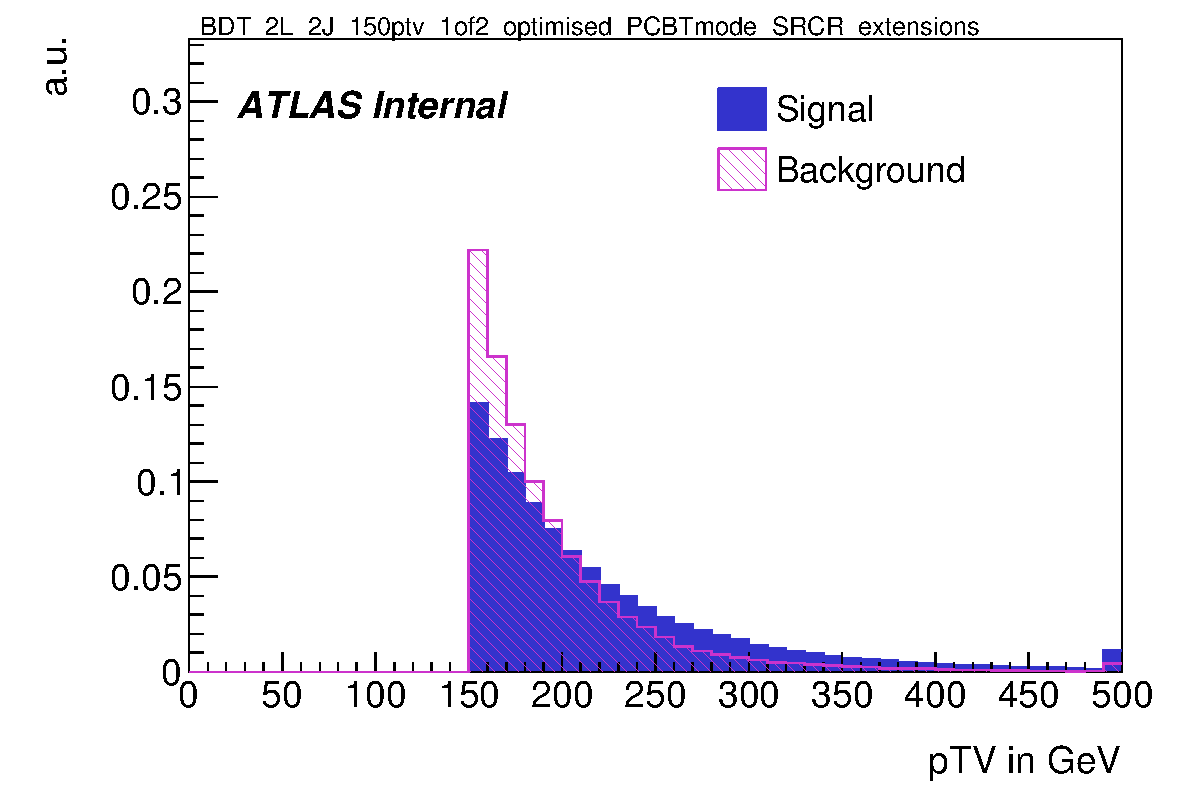
\includegraphics[width=0.33\linewidth]{2-lep-mva/Distr_SignalBackground_pTV_BDT_2L_2J_150ptv_1of2_optimised_PCBTmode_SRCR_extensions-eps-converted-to}}   
    \end{tabular}
    \caption{Input variables passed to the BDT for sum of all signal (blue) and sum of all background (red) samples in the 2 lepton channel for the 2 jet region with $p_{\text{T}}^{Z}>$150 {GeV} are shown. The signal and background templates are normalised to the same yield. The variable range for the training is restricted to contain 99\% of all signal events and the events in the overflow are included in the last bin.}
    \label{fig:bdtinputs2L2J150}
\end{figure}
